\chapter{Empirical study}
\label{chapter4}
The \textit{goal} of our empirical study is to evaluate the proposal of combining multiple models to improve accuracy of testing processes and to evaluate \textbf{RIP} as a tool to automatically crawl Android applications. We evaluate our proposal in terms of (i) the importance of combining orthogonal information from different models and (ii) the suitability of a multi-model testing tool, in the process of developing mobile applications. At the same time, we evaluate \textbf{RIP} in terms of (iii) RIP's ability to crawl native and hybrid Android apps, and (iv) RIP's ability to detect bugs and generate crashes. The \textit{context} of this study consists of (i) a set of 15  open source native APKs, (ii) a set of 20 hybrid APKs from the Google Play Store, and (iii) three baseline approaches for extracting models and crawl Android applications: DroidBot \cite{Li:ICSE17}, Firebase Test Lab Robo \cite{firebase} and Monkey \cite{monkey}.

The \textit{quality focus} of this study is the effectiveness of \textbf{RIP} to detect  states on both native and hybrid apps, reporting crashes and generating multi-models from these applications. To aid in achieving the goals of the study, the following research questions were formulated:

\begin{itemize}
	\item \textit{\textbf{RQ$_1$}}: \textit{Is the combination of multiple models useful to gather more information of an app under test?}
	\item \textit{\textbf{RQ$_2$}}: \textit{How accurate is the state discovery algorithm' implemented in RIP when compared to state-of-the art tools?}
	\item \textit{\textbf{RQ$_3$}}: \textit{Is RIP suitable to detect crashes and bugs in Android apps?}
\end{itemize}
 
Note that when answering the research questions we take into account hybrid and native Android apps. These two development strategies could be indistinguishable for final users of the apps, yet their are very different to crawl, analyze and build. \textbf{RIP has been designed to support both types of apps.}

\section{Context of the study}

A set of 15 native Android apps and 20 hybrid apps were downloaded from the Google Play Store and F-Droid. The native apps were randomly selected from F-Droid. In order to identify and download the set of hybrid apps, it was necessary to check the different hybrid frameworks showcases, find the APKs in the Google Play Store and then decompile the APKs to identify the presence of hybrid packages (\eg \verb|com.ionicframework|). Additionally, to verify that these apps contain web based GUI elements, the \textit{Show layout bounds} setting was activated in a device. With this option enabled, it is possible to visually identify native Android components in a device screen. Figure \ref{layoutBounds} shows that in native apps, this option draws red and blue lines around every graphical element. On the other hand, it can be seen that when this option is enabled in a hybrid app, none of these components is detected by the layout manager.

\begin{figure}[t]
	\centering
	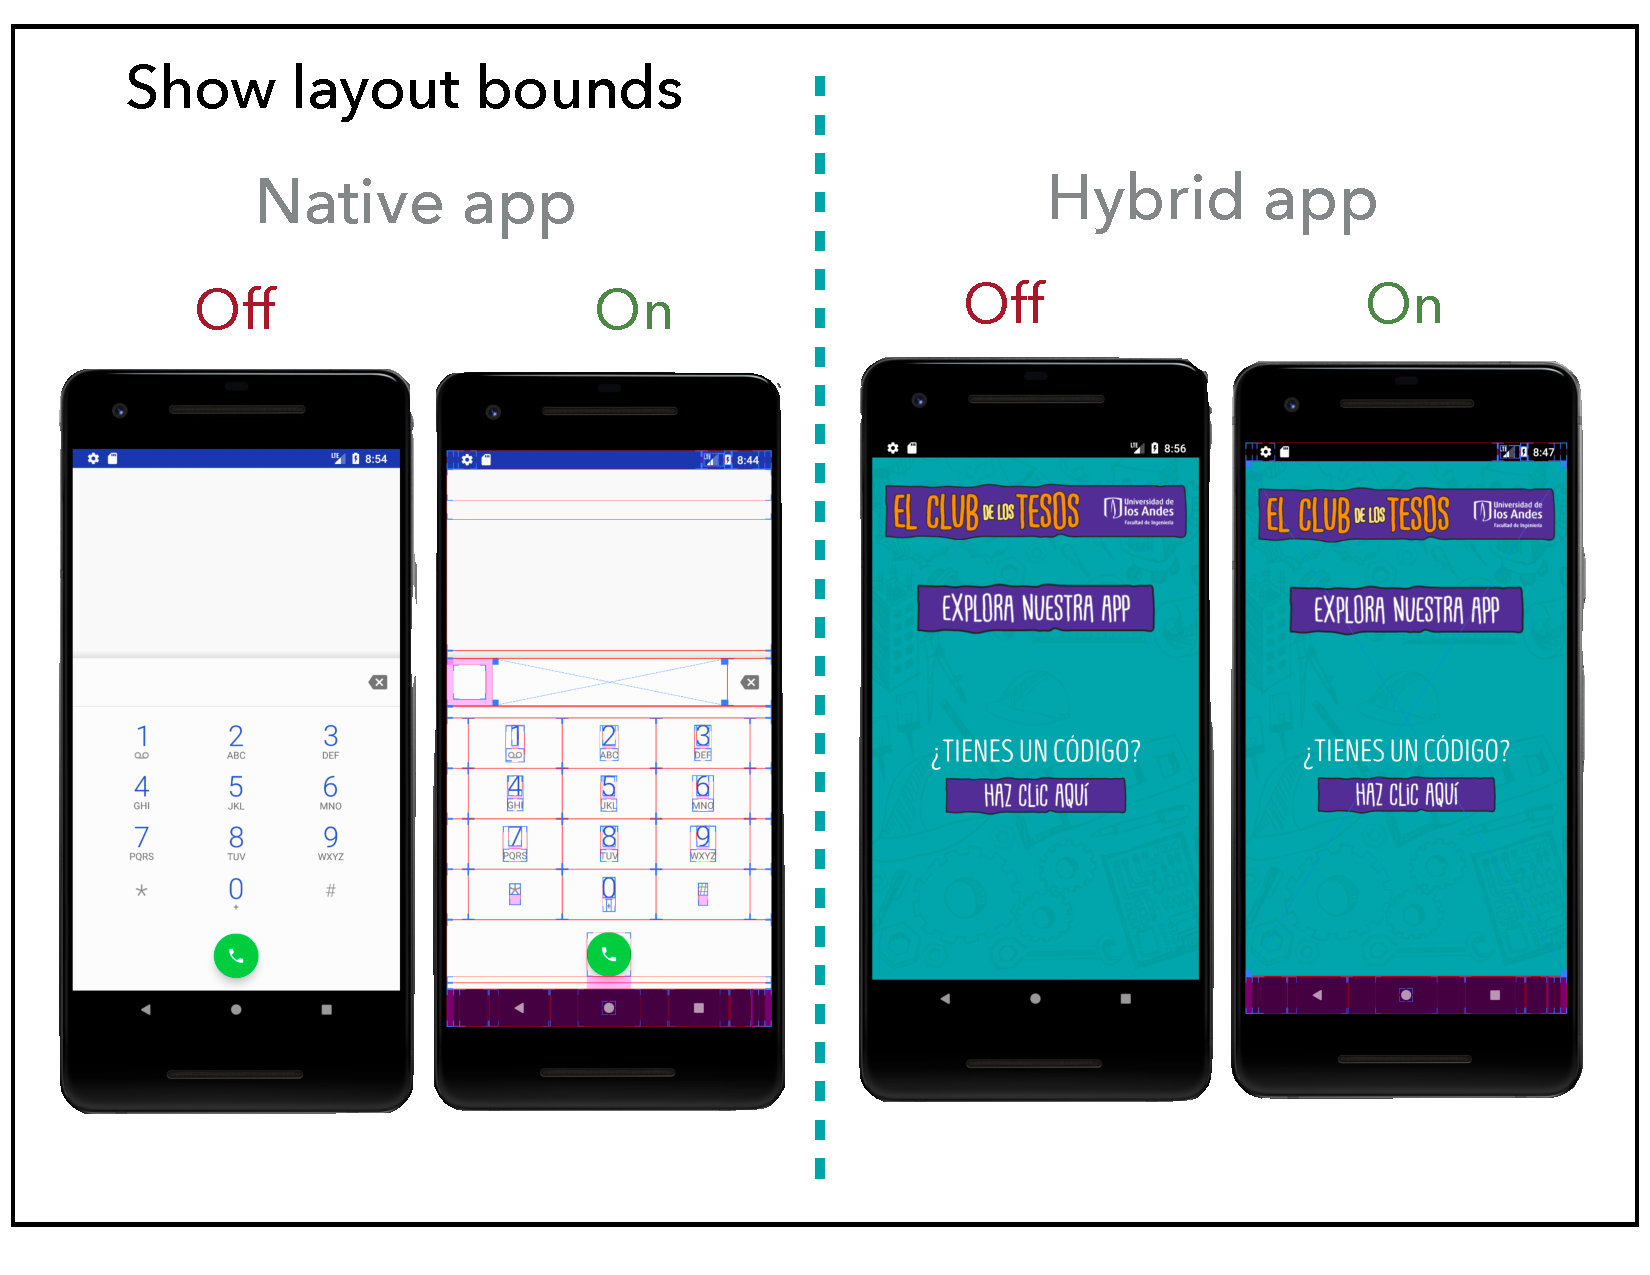
\includegraphics[width=1\textwidth]{img/layout.pdf}
	\vspace{-0.8cm}
	\caption{Enabling layout bounds detection in hybrid and native apps}
	\label{layoutBounds}
\end{figure} 


All the applications were installed and tested in an Android emulator for a \textit{Pixel 2} device with API 27 (Android 8.1 Oreo).  The screen proportions of the device are \verb|1080 x 1920| with 420\verb|dpi|.  The CPU/ABI of the device is a Google's API Intel Atom (x86) with 1.5 GB of RAM.

The detailed list of applications used during the study is presented in Table \ref{appsTable}

\begin{table*}[t]
	\centering
	\caption{List of applications used in the study}
	\label{appsTable}
	\begin{adjustbox}{width=\textwidth}
		\begin{tabular}{|c|c|c|c|c|l|}
			\hline
			\textbf{Name} & \textbf{Category} & \textbf{Size\tiny{(MB)}} & \textbf{Source} & \textbf{Tech} &\textbf{Package}  \\ \hline
			Amaze&Tools&5.8&F-Droid&Native&\small{com.amaze.filemanager}\\ \hline
			aMetro&Maps \& navigation& 2.62&F-Droid&Native&\small{org.ametro}\\ \hline
			Barcode Scanner&Tools&0.73&F-Droid&Native&\small{com.google.zxing.client.android}\\ \hline
			Materialistic&News \& Magazines&3.56&F-Droid&Native&\small{io.github.hidroh.materialistic}\\ \hline
			Minimal&Productivity&1.88&F-Droid&Native&\small{com.rubenroy.minimaltodo}\\ \hline
			Mysplash&Personalization&4.82&F-Droid&Native&\small{com.wangdaye.mysplash}\\ \hline
			Omni Notes&Productivity&4.82&F-Droid&Native&\small{it.feio.android.omninotes.foss}\\ \hline
			RadioDroid&Music \& audio&4.19&F-Droid&Native&\small{net.programmierecke.radiodroid2}\\ \hline
			Tasks&Productivity&6.29&F-Droid&Native&\small{org.tasks} \\ \hline
			Car Report&Auto \& Vehicles&2.93&F-Droid&Native&\small{me.kuehle.carreport}\\ \hline
			Calendar&Productivity& 6.08&F-Droid&Native&\small{com.simplemobiletools.calendar}\\ \hline
			Tusky&Social&2.93&F-Droid&Native&\small{com.keylesspalace.tusky}\\ \hline
			AnotherMonitor&Tools&0.2&F-Droid&Native&\small{org.anothermonitor}\\ \hline
			Antennapod&Video Players&5.87&F-Droid&Native&\small{de.danoeh.antennapod}\\ \hline
			Trolly&Shopping&0.03&F-Droid&Native&\small{caldwell.ben.trolly}\\ \hline
			McLaren Automotive&Auto \& Vehicles&60&Google P.&Hybrid&\small{com.mclaren.mclaren2019}\\ \hline
			Joule&Food \& Drink&95.3&Google P.&Hybrid&\small{com.chefsteps.circulator}\\ \hline
			Sworkit&Health \& Fitness&78.1&Google P.&Hybrid&\small{sworkitapp.sworkit.com}\\ \hline
			Untappd &Food \& Drink&44.4&Google P.&Hybrid&\small{com.untappdllc.app}\\ \hline
			Hockey Community&Sports&4.9&Google P.&Hybrid&\small{com.hockeycommunity.hc\_app}\\ \hline
			Tomatoid&Productivity&0.3&Google P.&Hybrid&\small{com.tomatoid.api}\\ \hline
			Mobimall&Libraries \& Demo&16.7&Google P.&Hybrid&\footnotesize{com.verbosetech.mobimall\textunderscore ionicdemo}\\ \hline
			Ionic Framework&Education&4.7&Google P.&Hybrid&\small{com.gsolution.ionicdemo}\\ \hline
			El club de los tesos&Education&15.8&Google P.&Hybrid&\small{uniandes.tsdl.tesosApp}\\ \hline
			IELTS PRACTICE&Education&2&Google P.&Hybrid&\footnotesize{com.examgroupapps.ieltslistening\textunderscore practice}\\ \hline
			TripCase &Travel \& Local&12.5&Google P.&Hybrid&\small{com.sabre.tripcase.android}\\ \hline
			Pacifica&Tools&38.2&Google P.&Hybrid&\small{icom.pacificalabs.pacifica}\\ \hline
			Tripline&Travel \& Local&1.9&Google P.&Hybrid&\small{inet.tripline}\\ \hline
			iTasca&Food \& Drink&3.8&Google P.&Hybrid&\small{it.tascadalmerita.iTasca}\\ \hline
			EcoAlimentate&Health \& Fitness&1.5&Google P.&Hybrid&\small{com.rma.ecoalimentate}\\ \hline
			Folver&Education&1.8&Google P.&Hybrid&\scriptsize{com.megabyteraingmail.com.theformulasolver}\\ \hline
			Hybrid Native&Libraries \& Demo&4&Google P.&Hybrid&\small{com.kathanshah.hybridnative}\\ \hline
			McDonald's &Food \& Drink&9.6&Google P.&Hybrid&\small{icom.clockwork.mcdonalds}\\ \hline
			Cordova ionic VR&Shopping&23.1&Google P.&Hybrid&\footnotesize{it.tangodev.cordovapluginvrviewsampleapp}\\ \hline
			Fashion Ecommerce&Libraries \& Demo&11&Google P.&Hybrid&\footnotesize{icom.vectorcoder.ionicecommerce.demo2}\\ \hline
		\end{tabular}
	\end{adjustbox}
\end{table*}



\section{\textbf{RQ$_1$} Combining multiple models to improve accuracy of testing processes}
To answer \textit{\textbf{RQ$_1$}}, we conducted a case study to show that combining the different models in an augmented model could improve the accuracy of testing processes. It means, we wanted to understand whether combining the models is useful to gather more knowledge of an app under test, and whether that knowledge could be used to generate more robust test cases. To this, we (i) extracted multi-models from 5 different Android apps which are listed in \tabref{experiment1}, and (ii) collected the following information using RIP:
\begin{table*}[]
	\centering
	\caption{General results obtained from multi-model extraction. \textbf{Abbreviations for column headings}. CR = Car Report, YLC = Your Local Weather, SC = Simple Calendar}
	\label{experiment1}
	\begin{adjustbox}{width=\textwidth}
	\begin{tabular}{|c|c|c|c|c|c|}
		\hline
		& \textbf{CR \cite{carReport}} & \textbf{Punky} & \textbf{YLC \cite{localWeather}} & \textbf{Tasks \cite{tasks}} & \textbf{SC \cite{simpleCalendar}}\\ \hline
		\textbf{Execution time (mins.)} &       4.6              &          4            &           6             &     5.3           &         4.8                 \\ \hline
		\textbf{Total number of states discovered}         &         51            &           30           &      31                  &     37           &          36                \\ \hline
		\textbf{States discovered due to contextual changes}               &     0                &         8             &             5           &          4      &            4              \\ \hline
		\textbf{Domain entities extracted}               &       21              &           4           &           23             &       17         &             20             \\ \hline
		\textbf{Attributes extracted}               &       63              &            96          &             27           &         60       &                  44        \\ \hline
	\end{tabular}
\end{adjustbox}
\end{table*}

\begin{itemize}
	\item  Execution time required to explore the applications until no more states were discovered,
	\item Total number of states discovered by triggering simulated user interactions and context events (ripping),
	\item States that were discovered due to contextual changes (ripping + context),
	\item Domain entities extracted from the apps,
	\item Attributes extracted from each domain entity
	
\end{itemize}

In the study we executed \textbf{RIP} in two modes: (i) ripping only mode, and (ii) ripping + contextual model execution. As reported in \tabref{experiment1}, when we added the contextual model,  we found new states in 4 out of 5 applications tested. This suggest that generating augmented models can improve software comprehension and  testing tasks for mobile apps, because different states are activated by combining individual models.

The first row of \tabref{experiment1} shows the execution time required to explore the applications until no more states were discovered. Second row includes total number of states discovered by triggering simulated user interactions and context events. Next row shows only the states that were discovered due to contextual changes. Based on the information of these two rows is easy to conclude that Car Report is an application that relays much less to contextual changes in comparison with Your local weather or Simple Calendar. In the case of Punky, changes due to context were triggered by Wi-Fi, Bluetooth and accelerometer interactions.

The Domain entities extracted' row refers to entities discovered. This number is directly correlated to the number of application views that contain text inputs, selectors and checkboxes. Each entity contains a set of attributes, whose sum correspond to the final row. 

Table \ref{experiment1} shows that information from each model is complementary and orthogonal.  For instance, applications that are highly dependent on sensors and networking connections have states that could not be discovered if contextual events are not considered.

\begin{tcolorbox}[title= \textit{\textbf{RQ$_1$}} Is the combination of multiple models useful to gather more information of an app under test?]
	Automatically extracting augmented models from Android apps enables better understanding of the apps. For modern mobile applications, ripping apps --- but based only on GUI exploration--- is not enough because they are context-aware. To that end, context, GUI, usage and domain models should be extracted and combined together to build more useful and comprehensive augmented models. 
\end{tcolorbox}

\section{\textbf{RQ$_2$} How accurate is the \textit{state discovery algorithm} implemented in RIP when compared to state-of-the art tools?}

A second case study was conducted to determine how RIP compares with existing tools in industry and academy. Table \ref{tools}  depicts the features of the tools. The state discovery algorithm of RIP includes (i) contextual changes, (ii) DFS based exploration and detection of hybrid or native components in applications, (iii) triggering monkey actions in the user interface and (iv) detection of states. Code example \ref{pseudocode} describes this algorithm.%\MARIO{Santiago, in section 3 there should a listing describing the algorihtm  in a pseudocode TODO}

\begin{table*}[h]
	\centering
	\caption{Industry and academy tool features}
	\label{tools}
	\begin{adjustbox}{width=0.8\textwidth}
		\begin{tabular}{|c|c|c|c|c|c|}
			\hline
			&\textbf{RIP}&\textbf{Monkey}&\textbf{Firebase}&\textbf{DroidBot}\\\hline
			GUI Ripping&\checkmark&&\checkmark&\checkmark\\\hline
			Contextual changes&\checkmark&&&\\\hline
			Random events&\checkmark&\checkmark&\checkmark&\checkmark\\\hline
			Model-based crawling (systematic)&\checkmark&&\checkmark&\checkmark\\\hline
			Works without instrumentation&\checkmark&\checkmark&\checkmark&\checkmark\\\hline
			State graph generation&\checkmark&&\checkmark&\checkmark\\\hline
			Crashes detection&\checkmark&&\checkmark&\\\hline
		\end{tabular}
	\end{adjustbox}
\end{table*}

\subsection{UI/Application Exerciser Monkey}

`Monkey is a program that runs on your emulator or device and generates pseudo-random streams of user events such as clicks, touches, or gestures, as well as a number of system-level events' \cite{monkey}. Monkey is part of the Android SDK and run from the command-line. Monkey was picked for the study because it (i) testers use it frequently to stress applications, (ii) it is part of the Android SDK and (iii) reports crashes and errors. `Is the most frequently used tool to test Android apps, partly because it is part of the Android developers toolkit and does not require any additional installation effort' \cite{Choudhary:ASE15}

The UI/Application Exerciser Monkey was executed with native and hybrid applications. Using the command \texttt{adb shell monkey -p <Package name> --throttle <Time between events> -v <Number of events>}. For each application, 500, 1000 and 2000 events were executed in order to identify a relation between this number and the number of states discovered.

\textbf{Native applications.} The results of Monkey executions over native applications are presented in Figure \ref{monkeyNative}. The average of discovered activities with 500 events was 2.2, with 1,000 events was 2.6 and with 2,000 events was 2.9. In order to determine if there is a difference in the number of activities found for each quantity of events, as data was obtained from the same applications and sample sizes are small (n=15), it must be performed a nonparametric test for related samples therefore, a Friedman test was performed to compare the three series.

The null hypothesis for the test is that there are no difference between the number of activities found by Monkey with 500, 1,000 and 2,000. The alternative hypothesis is that at least with one of the number of events changes the number of activities found by Monkey.

The p value obtained was 0.42 hence the null hypothesis is not rejected,  using an alpha of 5\% it was concluded that there is no difference in the number of activities explored by Monkey ranging by 500, 1,000 and 2,000 events.
%a Wilcoxon signed ranks test was performed. \MARIO{why wilcoxon? There are three series to be compared? Why are you talking of pairs? Before running paired tests  (i.e., post hoc tests) there should be a test including all the series (e.g., Friedman or Kruskal-Wallis)}  As can be seen in \tabref{WilcoxonMonkey}, there was no difference between each pair of events, which implies that with a significance of 10\% \MARIO{What do you mean with a significance of 10\&? what was the alpha used in the test?}, the number of events performed by Monkey (500, 1,000, 2,000) does not modify the number of activities found.
\begin{figure}[t]
	\centering
	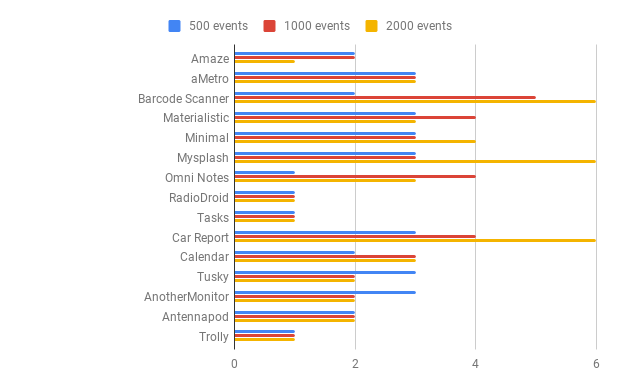
\includegraphics[width=0.9\textwidth]{img/monkeyNative.png}
	\caption{Number of discovered activities by Monkey executions with 500, 1,000 and 2,000 events over native applications}
	
	\label{monkeyNative}
\end{figure} 

%\begin{table*}[h]
%	\centering
%	\caption{Results of Wilcoxon signed ranks test for the number of activities found in native applications of Monkey executions ranging the number of events} \MARIO{why 5 and 6 samples? There should be 15 data per series (one datum per app)}
%	\label{WilcoxonMonkey}
%	\begin{adjustbox}{width=0.7\textwidth}
%		\begin{tabular}{|c|c|c|c|c|}
%			\hline
%			\textbf{Relation of events}&\textbf{500 - 1,000} & \textbf{500 - 2,000} & \textbf{1,000 - 2,000} \\\hline
%			\textbf{n samples}& 5 & 6 & 6 \\\hline
%			\textbf{Significance}& 10\% & 10\% & 10\% \\\hline
%			\textbf{T obtained value}& 1 & 3 & 3 \\\hline
%			\textbf{T critical value}& 0 & 2 & 2 \\\hline
%			\textbf{Diference?}& No & No & No \\\hline

%		\end{tabular}
%	\end{adjustbox}
%\end{table*}

\textbf{Hybrid applications.} Even though Monkey does not advertise special capabilities for hybrid applications, it was able to execute random events in the user interface. During the tests execution, it was evident that these random interactions made changes in the interface. Monkey is not designed to perform contextual changes in the application, however, due to the randomness of the GUI changes, in some rare cases it turned off or on airplane mode and connectivity settings.

Figure \ref{monkeyHybrid} Presents the discovered activities by Monkey with 500, 1000 and 2000 events. What this graph shows, is that almost for every app, the number of discovered activities was the same: 1. The explanation of this behavior comes from the conception of the hybrid app, with a single activity with a web view. The applications that contains more than a single activity are special cases that have multiple web views in different activities.

This experiment shows that even though Monkey made changes in the application, it only considers new activities as new states, it does not have a states memory. Monkey was successful interacting with the app, however, for hybrid apps, there is no way to determine how many states it visited if is not complemented with additional software.

\begin{figure}[t]
	\centering
	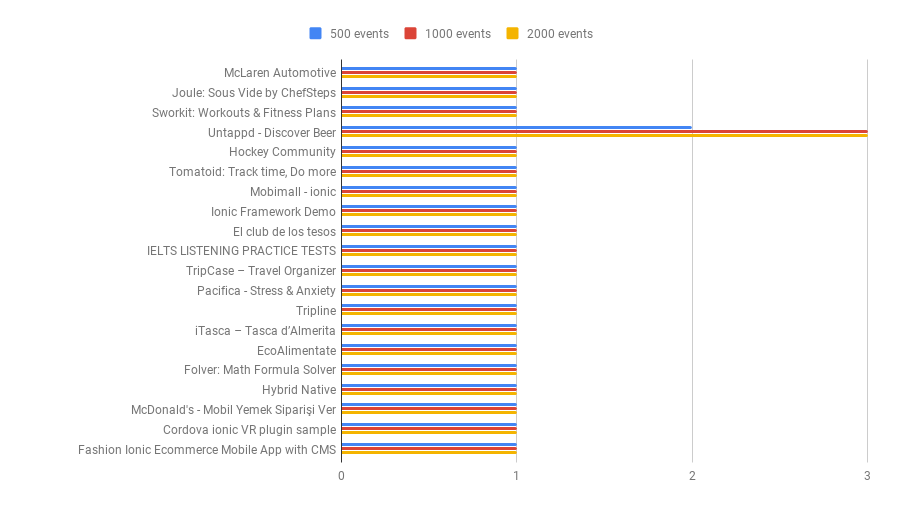
\includegraphics[width=0.9\textwidth]{img/monkeyHybrid.png}
	\caption{Number of discovered activities by Monkey executions with 500, 1,000 and 2,000 events over hybrid applications}
	
	\label{monkeyHybrid}
\end{figure} 

\textbf{Summary for UI/Application Exerciser Monkey.} The experiments show that Monkey is capable of identify different activities in native applications. However, changing the number of events performed does not make a significant difference in the number of activities encountered. Also, the average activity coverage of Monkey is 38\% in native applications, which suggests that a completely random discovery approach could be improved by a model-based approach.

As for hybrid applications, Monkey is not capable of reporting the number of states discovered insomuch as it only report activities. Monkey lacks ripping capabilities and does not aggregate results, which make analysis of its execution a hard task; a developer must follow all the events and activities to determine the states discovered by this random tool.

Based on the experiments conducted with this tool, we determined the importance of trigger random events in hybrid applications. This is a qualitative conclusion and tests to analyze quantitatively the importance of randomness in hybrid applications is part of our future work.

\subsection{Firebase Test Lab Robo Test}

Firebase Test Lab \cite{firebase} is one of the industry leaders in mobile testing. It has a cloud-based app-testing infrastructure that enables concurrent execution of tests with and without instrumentation. Firebase Test Lab Robo Test is one of their services: `Robo test analyzes the structure of your app's UI and then explores it methodically, automatically simulating user activities' \cite{firebase}. It cloud service allows testers to run Robo test on virtual and physical devices in parallel, detecting crashes and performance issues.

Firebase Test Lab was chosen in the study because it is the Google's flagship product in automated testing.

For each application, a Robo Test was configured and run. To configure each test, the developer must choose the specific device: in our case, \textit{Google Pixel's 2 API 27} was selected. The test recorded the number of actions performed during the exploration, the number of activities covered, the number of distinct screens visited and the duration. Is worth remembering that Firebase Test Lab is a cloud service and all the infrastructure is managed by Google. To that end, this service is very easy to use and the only requirement for the final user is to have the APK that he wants to test.

\textbf{Native applications.} The native applications were submitted to the service, and after each execution finished, Google sent an email informing the final result for every test. \tabref{FirebaseNative} presents the results of running Firebase Test Lab, indicating the duration, number of actions, activities and screens for the applications.  
\begin{table*}[t]
	\centering
	\caption{Results of running Firebase Test Lab on native applications}
	\label{FirebaseNative}
	\begin{adjustbox}{width=0.8\textwidth}
		\begin{tabular}{|c|c|c|c|c|}
			\hline
			\textbf{Application} & \textbf{Duration (s)} & \textbf{Actions} & \textbf{Activities} & \textbf{Screens} \\\hline
			Amaze & 314 & 268 & 1 & 120 \\\hline
			aMetro & 309 & 343 & 4 & 73 \\\hline
			Barcode Scanner & 258 & 204 & 7 & 27 \\\hline
			Materialistic & 301 & 87 & 6 & 28 \\\hline
			Minimal & 304 & 200 & 4 & 26 \\\hline
			Mysplash & 313 & 68 & 6 & 23 \\\hline
			Omni Notes & 25 & 8 & 1 & 3 \\\hline
			RadioDroid & 313 & 122 & 1 & 79 \\\hline
			Tasks & 303 & 227 & 6 & 90 \\\hline
			Car Report & 305 & 202 & 5 & 37 \\\hline
			Calendar & 304 & 205 & 6 & 64 \\\hline
			Tusky & 33 & 12 & 1 & 4 \\\hline
			AnotherMonitor & 318 & 133 & 4 & 19 \\\hline
			Antennapod & 314 & 141 & 5 & 59 \\\hline
			Trolly & 11 & 7 & 1 & 1 \\\hline
		\end{tabular}
	\end{adjustbox}
\end{table*}
Figure \ref{firebase} depicts the outcomes of the execution for a specific app, including a full video of the whole crawling process, aggregated statistics and a very detailed crawl graph. This graph shows the different screens connected with edges associated to clicks and button pressings. The applications that seem to have a low number of screens (\eg Trolly: 1, Omni Notes: 3) have login and authentication activities in the applications. In these scenarios, Testlab is unable to automatically create users or introduce credentials, and does not explore more than the initial screens. 

\begin{figure}[t]
	\centering
	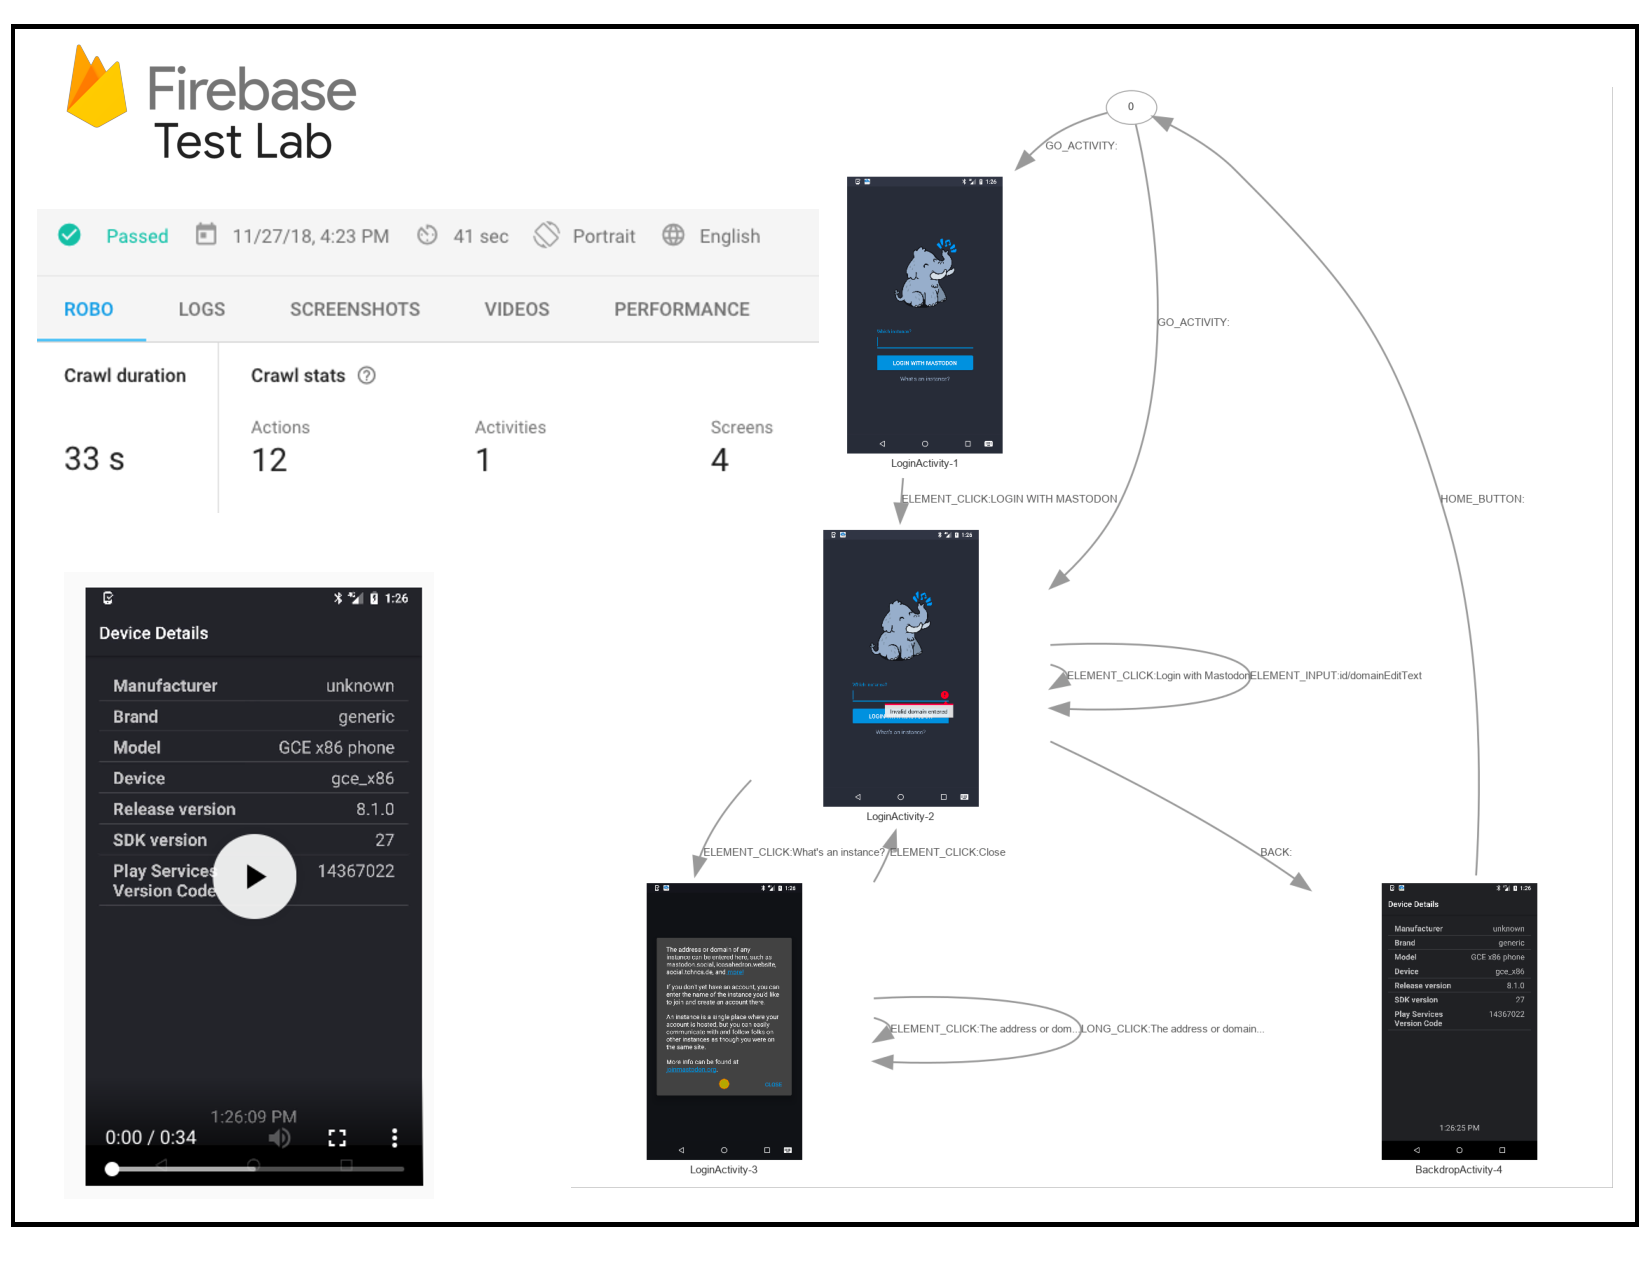
\includegraphics[width=1\textwidth]{img/firebase.pdf}
	\caption{Firebase Test Lab: Results of a Robo Test for a single native app}
	
	\label{firebase}
\end{figure} 

\textbf{Hybrid applications.} Regarding hybrid applications, Firebase Test Lab's behavior was entirely different from its native execution \tabref{FirebaseHybrid}. In almost all the applications, the number of activities discovered was 1 because hybrid apps usually do not have more than one activity. There are two groups of apps: those with a number of screens greater than 60 and those with a number of screens lower than 10. Examining carefully those applications with a big number of screens found, we identified that Firebase classified screens with animations as multiple screens; one of this cases is presented in Figure \ref{multipleScreens}.  In this figure, an animation is running in the background of the screen, the animation is continuously changing. The Robo Test is visually detecting updates in the screen, and as the frames change, it detects new screens of the application.

\textbf{Summary of Firebase Test Lab Robo Test.} Firebase Test Lab is a easy to use service that explored native and hybrid applications in a short time. It detected several different screen in hybrid applications, however, it did not explore correctly hybrid applications. In none of them it was able to detect the states correctly and build the crawl graph.

\begin{table*}[t]
\centering
\caption{Results of running Firebase Test Lab on hybrid applications}
\label{FirebaseHybrid}
\begin{adjustbox}{width=0.9\textwidth}
	\begin{tabular}{|c|c|c|c|c|}
		\hline
		\textbf{Application} & \textbf{Duration (s)} & \textbf{Actions} & \textbf{Activities} & \textbf{Screens} \\\hline
		McLaren Automotive & 15 & 4 & 1 & 3 \\\hline
		Joule & 306 & 194 & 1 & 146 \\\hline
		Sworkit & 163 & 63 & 1 & 6 \\\hline
		Untappd & 9 & 6 & 1 & 2 \\\hline
		Hockey Community & 322 & 20 & 1 & 3 \\\hline
		Tomatoid & 86 & 70 & 1 & 3 \\\hline
		Mobimall & 9 & 8 & 1 & 2 \\\hline
		Ionic Framework & 37 & 10 & 1 & 3 \\\hline
		El club de los tesos & 11 & 4 & 1 & 3 \\\hline
		IELTS PRACTICE & 253 & 79 & 2 & 5 \\\hline
		TripCase & 26 & 15 & 1 & 3 \\\hline
		Pacifica & 282 & 235 & 4 & 62 \\\hline
		Tripline & 82 & 24 & 1 & 4 \\\hline
		iTasca & 79 & 17 & 1 & 3 \\\hline
		EcoAlimentate & 5 & 4 & 1 & 2 \\\hline
		Folver & 74 & 22 & 1 & 6 \\\hline
		Hybrid Native & 144 & 31 & 2 & 9 \\\hline
		McDonald's & 91 & 28 & 1 & 3 \\\hline
		Cordova ionic VR & 80 & 21 & 2 & 9 \\\hline
		Fashion Ecommerce & 72 & 17 & 1 & 2 \\\hline
	\end{tabular}
\end{adjustbox}
\end{table*}
% \begin{figure}[t]
%	\centering
%	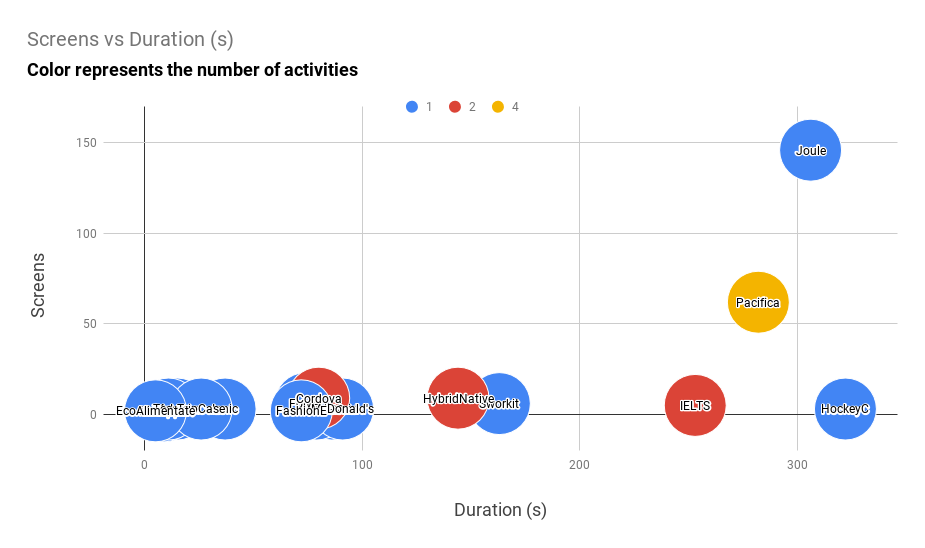
\includegraphics[width=1\textwidth]{img/screensVsDurationFhybrid.png}
%	\caption{Firebase: Number of screens vs duration\textit{ Color represents the number of detected activities}}	
%	\label{screensVsDurationFhybrid}
%\end{figure} 
\begin{figure}[t]
	\centering
	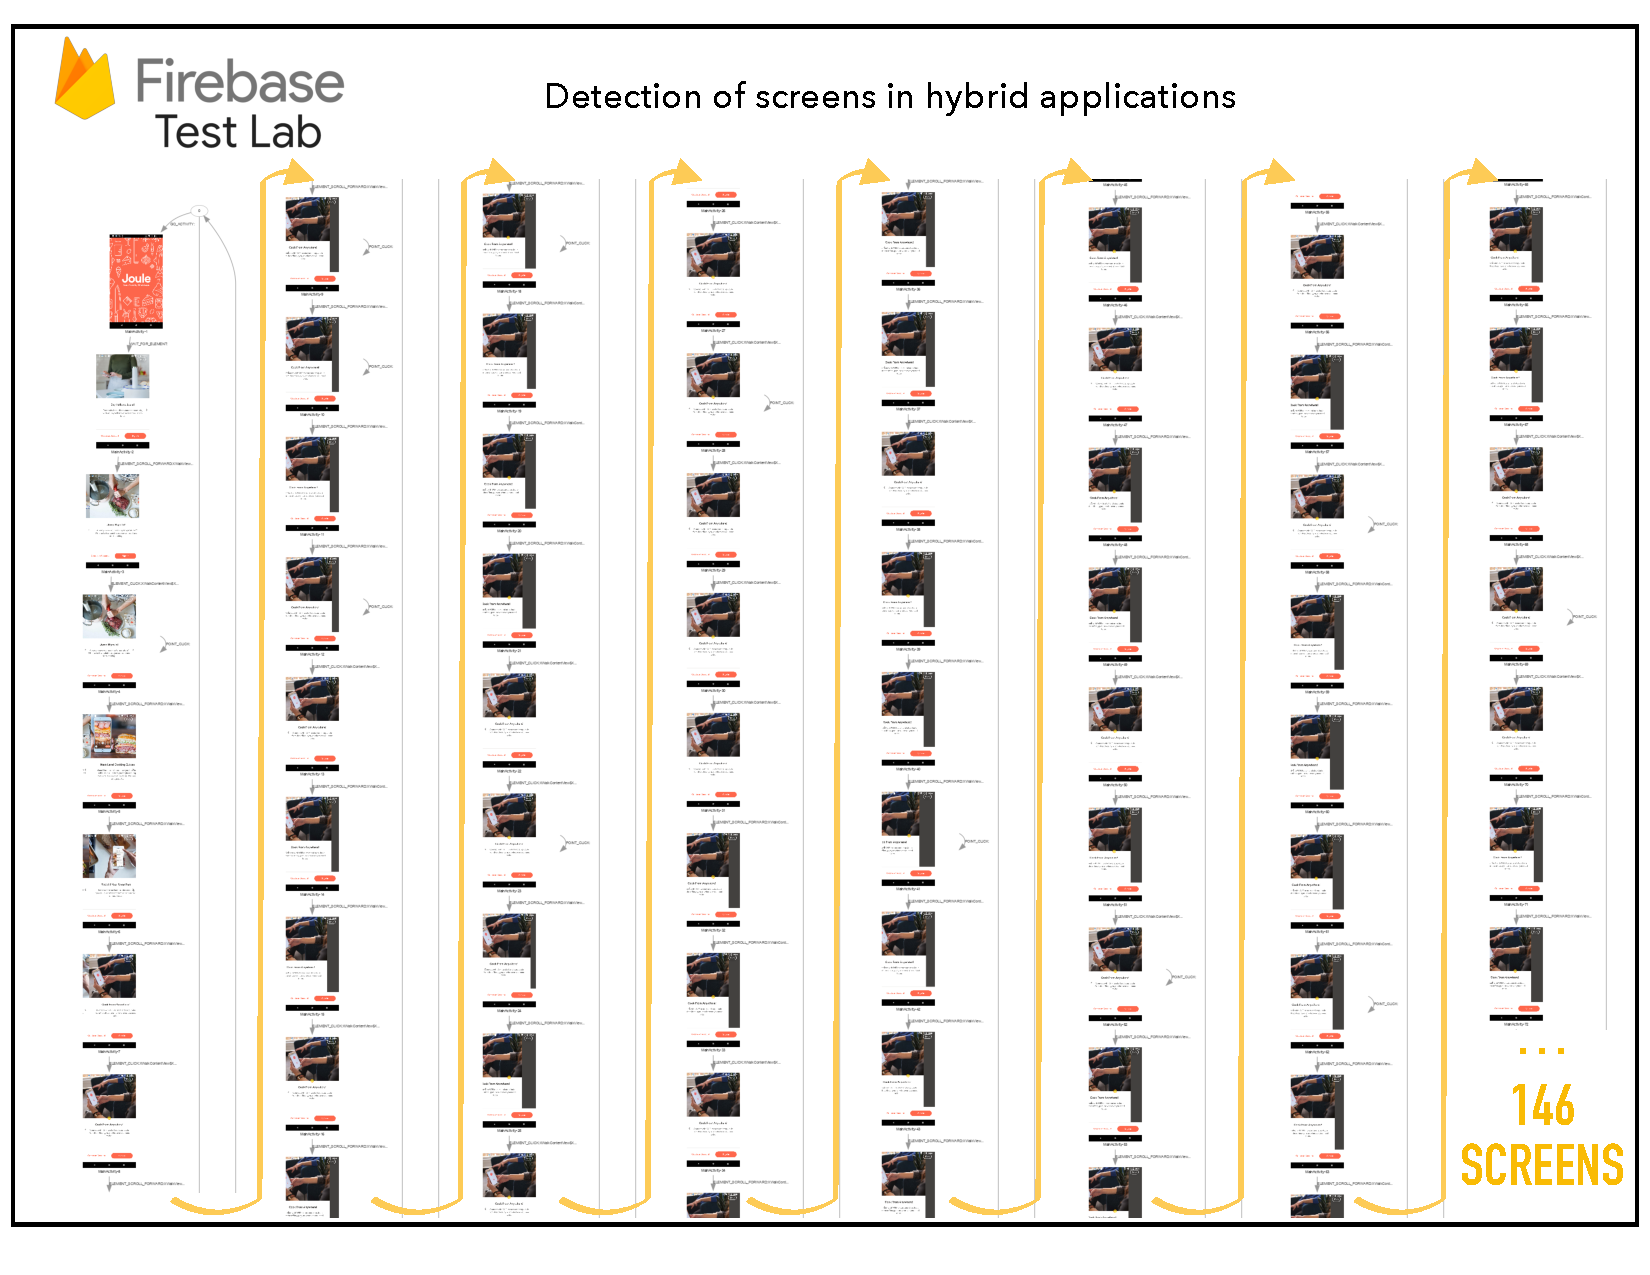
\includegraphics[width=1\textwidth]{img/multipleScreens.pdf}
	\vspace{-0.8cm}
	\caption{For some hybrid apps with animations, Firebase detect the same state multiple times and reports a unreal number of screens}
	
	\label{multipleScreens}
\end{figure} 



\subsection{DroidBot}

DroidBot \cite{Li:ICSE17} is a tool that uses a model-based strategy to automatically explore mobile GUIs. It generates inputs and a transition model between different states of the application. One of the main features of DroidBot is that it does not require app instrumentation and is mean to run in almost any Android device. DroidBot is open source and publicly available \cite{droidbotRepo}.
It was choose as a baseline for the study because its availability and effectiveness exploring mobile applications.

DroidBot was executed running the command \texttt{droidbot <APK name> -o <Output folder> -is\_emulator -random} for the complete set of applications. The \texttt{-random}  flas was used to add randomness to input events and the \texttt{-is\_emulator}  flag was required for running droidbot on virtual devices . The exploration strategy used was \textit{dfs\_greedy} which explores UI using a greedy depth-first strategy. DroidBot implements other search strategies (\eg \textit{dfs\_naive}, \textit{bfs\_naive}, \textit{bfs\_greedy}), but  \textit{dfs\_greedy} was chosen because this strategy is a better approximation when trying to explore completely a tree.

For each tested application DroidBot generates a UTG (\textit{UI Transition Graph}), screen shots of the states and an HTML report that includes the time spent, number of input events, number of UTG states, number of UTG edges and activity coverage.

\textbf{Native applications.} The results of DroidBot on native applications are shown in \tabref{DroidNative}, the average activity coverage is 52\% and  the average duration is 73 minutes. Also, the number of input events rounds 990 and the discovered states range between 37 and 874 with a standard deviation of 218. It can be seen that the average duration of the test is more than 10 times the maximum duration of a Robo test in Firebase. Also, from the state graphs generated it can be noticed that many of the states registered by DroidBot are almost the same, they share the same layout but only the content in the fields changes. For example, the most repeated case is in a login form, each time DroidBot changes the input fields a state is reported. Moreover, if DroidBot leaves the login view and comes back after, it reports again all the states generated from login view.

\begin{table*}[t]
	\centering
	\caption{Results of running DroidBot  on native applications  \textbf{Abbreviations for column headings}. \textit{RA} = Registered activities in the app, \textit{FA} = Found activities during exploration, \textit{AC} = Activity coverage, \textit{Time(s)} = Time of execution, Input events = Number of input events generated, \textit{UTG states} = UI Transition Graph States, \textit{UTG edges} = UI Transition graph edges}
	\label{DroidNative}
	\begin{adjustbox}{width=\textwidth}
		\begin{tabular}{|c|c|c|c|c|c|c|c|}
			\hline
			\textbf{App} & \textbf{RA} & \textbf{FA} & \textbf{AC} & \textbf{Time(s)} & \textbf{Input events} & \textbf{UTG states} & \textbf{UTG edges} \\\hline
			Amaze & 6 & 2 & 0.33 & 4492 & 996 & 295 & 453 \\\hline
			aMetro & 6 & 4 & 0.66 & 3966 & 998 & 108 & 248 \\\hline
			Barcode Scanner & 9 & 7 & 0.77 & 4173 & 997 & 49 & 106 \\\hline
			Material Notes & 23 & 6 & 0.26 & 5944 & 990 & 120 & 345 \\\hline
			Minimal & 5 & 4 & 0.8 & 3756 & 997 & 150 & 342 \\\hline
			Mysplash & 20 & 7 & 0.35 & 6796 & 995 & 221 & 489 \\\hline
			Omni Notes & 17 & 4 & 0.23 & 4238 & 992 & 196 & 405\\\hline
			RadioDroid & 2 & 1 & 0.5 & 3959 & 990 & 453 & 548\\\hline
			Tasks & 38 & 5 & 0.13 & 3437 & 997 & 69 & 116\\\hline
			Car Report & 8 & 7 & 0.87 & 4607 & 997 & 254 & 402 \\\hline
			Calendar & 12 & 7 & 0.58 & 4068 & 996 & 227 & 313\\\hline
			Tusky & 21 & 1 & 0.04 & 4754 & 996 & 16 & 37 \\\hline
			AnotherMonitor & 4 & 4 & 1 & 3437 & 995 & 819 & 874\\\hline
			Antennapod & 20 & 7 & 0.35 & 4434 & 997 & 328 & 518\\\hline
			Trolly & 2 & 2 & 1 & 3745 & 992 & 35 & 89 \\\hline
		\end{tabular}
	\end{adjustbox}
\end{table*}

\textbf{Hybrid applications.} The results of running DroidBot on hybrid applications are shown in \tabref{DroidHybrid}, it can be noticed that even though there are multiple registered activities in most of the applications, only one is discovered by the tool. This is due to the fact that the hybrid applications use a Web View which encapsulates the GUI components using, in most of the cases, only one activity.

Moreover, the average duration of the test was 68 minutes, the number of input events ranges between 723 and 998, and the average number of discovered states is 94.1. However, from the state graphs it can be seen that as DroidBot is unable to analyze the Web View, it keeps exploring outer applications like Facebook or Google (accessing to these services in the authentication screen). Also, DroidBot does not report only different states, we manually counted the number of repeated and outer application states and reported them as false positives. It was estimated that the 67.1\% of the states discovered correspond to false positives. As can be seen in Figure \ref{repeated}, extracted from a state graph generated by DroidBot, there are several states reported that share the same view.

\begin{figure}[t]
	\centering
	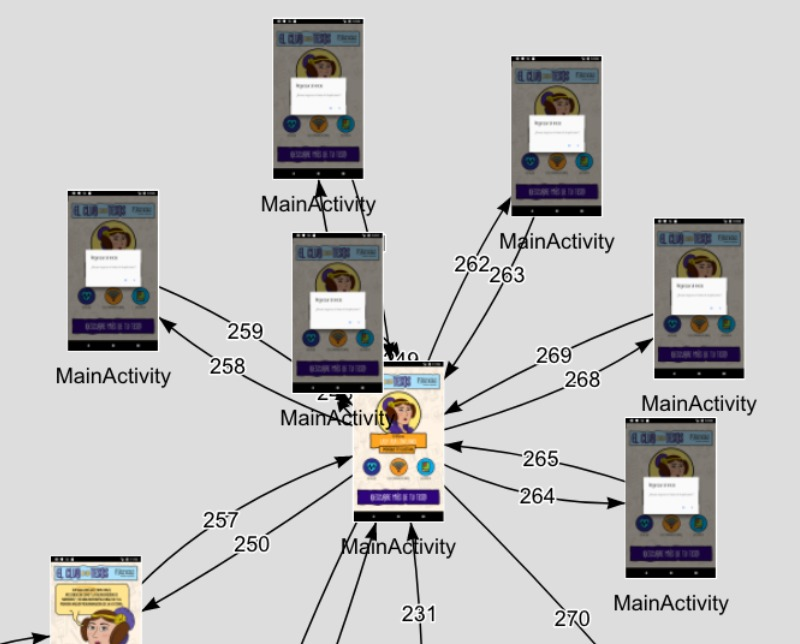
\includegraphics[width=0.8\textwidth]{img/exRepeated.png}
	\caption{Example of repeated states discovered by DroidBot}
	
	\label{repeated}
\end{figure} 

\begin{table*}[h]
	\centering
	\caption{Results of running DroidBot  on hybrid applications  \textbf{Abbreviations for column headings}. \textit{RA} = Registered activities in the app, \textit{FA} = Found activities during exploration, \textit{AC} = Activity coverage, \textit{Time(s)} = Time of execution, Input events = Number of input events generated, \textit{UTG states} = UI Transition Graph States, \textit{UTG edges} = UI Transition graph edges, \textit{FP States} = False positive states discovered.}
	\label{DroidHybrid}
	\begin{adjustbox}{width=\textwidth}
		\begin{tabular}{|c|c|c|c|c|c|c|c|c|}
			\hline
			\textbf{App} & \textbf{RA} & \textbf{FA} & \textbf{AC} & \textbf{Time(s)} & \textbf{Input events} & \textbf{UTG states} & \textbf{UTG edges} & \textbf{FP States}\\\hline
			McLaren Automotive & 6 & 1 & 0.16 & 3042 & 723 & 70 & 127 & 50 \\\hline
			Joule & 8 & 1 & 0.12 & 4792 & 997 & 65 & 120 & 49 \\\hline
			Sworkit & 14 & 2 & 0.14 & 8270 & 996 & 87 & 200 & 65 \\\hline
			Untappd & 11 & 2 & 0.18 & 3849 & 997 & 76 & 154 & 32 \\\hline
			Hockey Community & 17 & 2 & 0.11 & 3652 & 996 & 143 & 360 & 129 \\\hline
			Tomatoid & 1 & 1 & 1 & 3835 & 989 & 112 & 183 & 80 \\\hline
			Mobimall & 12 & 1 & 0.08 & 3508 & 997 & 174 & 388 & 155\\\hline
			Ionic Framework & 1 & 1 & 1 & 3410 & 997 & 256 & 558 & 254\\\hline
			El club de los tesos & 1 & 1 & 1 & 4035 & 997 & 32 & 99 & 14\\\hline
			IELTS PRACTICE & 2 & 2 & 1 & 3782 & 998 & 86 & 229 & 79\\\hline
			TripCase & 14 & 2 & 0.14 & 4072 & 992 & 142 & 240 & 122\\\hline
			Pacifica & 10 & 2 & 0.2 & 4005 & 993 & 116 & 301 & 107\\\hline
			Tripline & 3 & 1 & 0.33 & 3953 & 997 & 59 & 175 & 39\\\hline
			iTasca & 1 & 1 & 1 & 4179 & 997 & 61 & 129 & 49\\\hline
			EcoAlimentate & 1 & 1 & 1 & 3733 & 997 & 8 & 19 & 4\\\hline
			Folver & 4 & 1 & 0.25 & 3654 & 997 & 32 & 93 & 15\\\hline
			Hybrid Native & 1 & 1 & 1 & 3383 & 989 & 36 & 78 & 22\\\hline
			McDonald's & 5 & 1 & 0.2 & 4012 & 997 & 28 & 63 & 10\\\hline
			Cordova ionic VR & 3 & 1 & 0.33 & 3573 & 997 & 289 & 593 & 219\\\hline
			Fashion Ecommerce & 18 & 1 & 0.05 & 5105 & 997 & 10 & 19 & 0\\\hline
		\end{tabular}
	\end{adjustbox}
\end{table*}

\textbf{Summary for DroidBot.} DroidBot is able to generate a state graph from the ripping, it also reports the number of states discovered and its transitions. In native applications, it obtains an average activity coverage of 52\% on native applications, which is higher to the obtained by Firebase (44\%) and Monkey (38\%). However, the time spent in the test is more than 10 times the maximum duration of a Robo test in Firebase, this opens the possibility to find new approaches of ripping that increase the activity coverage in less time.  

As for hybrid applications, DroidBot is unable to analyze the Web View; therefore, it runs out of the main application generating a lot of states that does not refer to the application under test, and does not report the number of different states generating a large number of false positive states (67.1\%). 
\subsection{RIP}
We also analyzed the apps with our proposed tool, \textbf{RIP}.
 
\textbf{Native applications.} In order to compare RIP with Firebase and DroidBot, Table \ref{comparisonRIP} presents the average activity coverage, average number of states discovered, standard deviation of the number of states discovered, the average duration of the tests and the average number of new states discovered when applying contextual changes. It can be noticed that the higher activity coverage is reached by DroidBot (50.15\%) however, its average duration is about 17 times higher than Firebase and 14 times higher than RIP. The average number of states found by DroidBot is 5 times higher than Firebase and 7 times higher than RIP. 
Nevertheless, neither DroidBot nor Firebase apply contextual changes in the exploration of states. With contextual changes RIP reported 6.33 new states discovered on average.

RIP exploration algorithm was behind Firebase and DroidBot, however, enabling contextual changes in exploration allows \textbf{RIP} to find states that these tools are not able to detect.

Monkey was not included in this comparison because Monkey only reports different activities reached and does not rip the applications, it only triggers random events during the execution, and records in a log the activities found and the events triggered. From monkey's execution, it was valuable to see that its random approach sometimes toggle rare settings, that were hardly discovered from systematic approaches. This random exploration is very useful to detect crashes, however, is not  useful  at all for building a multi-model because it is difficulty to reproduce large and unguided scenarios generated by Monkey.

\begin{table*}[t]
	\centering
	\caption{Comparison in native applications between RIP, DroidBot and Firebase. \textbf{Abbreviations for row headings}. \textit{Std states} = Standard deviation of the number of states discovered,  \textit{\# States CC} = Number of states discovered when applying contextual changes. }
	\label{comparisonRIP}
	\begin{adjustbox}{width=0.6\textwidth}
		\begin{tabular}{|c|c|c|c|c|}
			\hline
			\textbf{Average metric}&\textbf{RIP} & \textbf{DroidBot} & \textbf{Firebase} \\\hline
			\textbf{Activity coverage}& 34.97\% & 50.15\% & 44.07\% \\\hline
			\textbf{\# States}& 28.06 & 222.66 & 43.53 \\\hline
			\textbf{Std states}& 24.63 & 204.83 & 35.55 \\\hline
			\textbf{Duration (min)}& 4.93 & 73.11 & 4.13 \\\hline
			\textbf{\# States CC}& 6.33 & - & - \\\hline
			
		\end{tabular}
	\end{adjustbox}
\end{table*}


\textbf{Hybrid applications.} In order to compare the state discovery algorithm implemented in RIP with Firebase and DroidBot (true positives only), we recorded the number of states discovered by each tool.  As it can be seen in Figure \ref{ripRad}, RIP detects a larger number of states almost in all applications compared to DroidBot and Firebase. 

It can be observed from \tabref{comparisonRIPHybrid} that the average number of true positive states discovered by RIP is 50.1, without outer applications or repeated states. Also, the average duration of RIP was 7.31 minutes which is 10 times less than the average duration of DroidBot. The number of states discovered by Firebase is 3 times lower than RIP's. Finally, in hybrid applications the only tool able to do contextual changes and detect new states generated is RIP, and it found in average 5.6 new states with this changes. 

The comparison of RIP vs Firebase performance is presented in Figure \ref{ripFirebase}. RIP was able to extract a complete graph from the hybrid application explored, including all the views and screens of the application. Firebase Test Lab opened the application, detected the splash view, and then the main screen of the application. After that, Firebase was unable to detect the components of the application. Related to hybrid apps exploration, RIP is superior.


\begin{figure}[t]
	\centering
	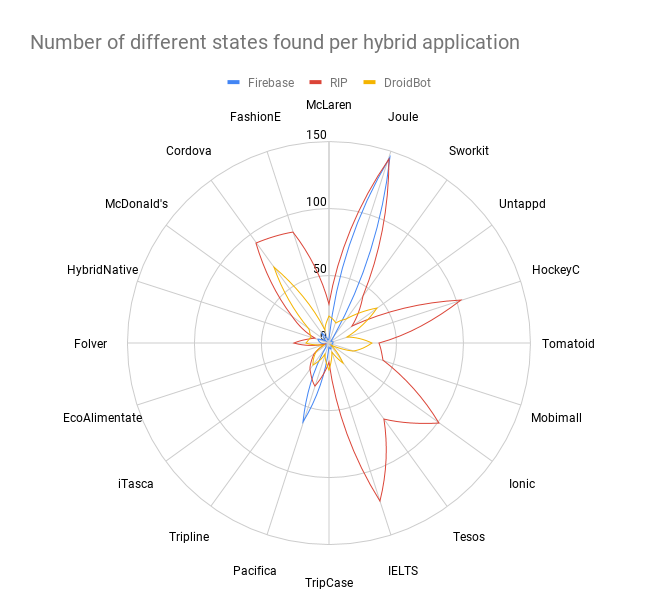
\includegraphics[width=1.1\textwidth]{img/ripRadComp.png}
	\vspace{-0.8cm}
	\caption{Comparison of the number of different states discovered on hybrid applications between RIP, Firebase and DroidBot}
	
	\label{ripRad}
\end{figure} 

\begin{table*}[t]
	\centering
	\caption{Comparison in hybrid applications between RIP, DroidBot and Firebase. \textbf{Abbreviations for row headings}. \textit{Std states} = Standard deviation of the number of states discovered,  \textit{\# States CC} = Number of states discovered when applying contextual changes, \textit{ \# TP states} = Number of different states discovered, \textit{FP states percentage} = Percentage of repeated or outer application or repeated states discovered. }
	\label{comparisonRIPHybrid}
	\begin{adjustbox}{width=0.6\textwidth}
		\begin{tabular}{|c|c|c|c|c|}
			\hline
			\textbf{Average metric}&\textbf{RIP} & \textbf{DroidBot} & \textbf{Firebase} \\\hline
			\textbf{\# States}& 52.6 & 94.1 & 13.95 \\\hline
			\textbf{Std states}& 39.29 & 76.16 & 33.74 \\\hline
			\textbf{\# TP States}& 50.1 & 19.4 & 12.7 \\\hline
			\textbf{Duration (min)}& 7.31 & 68.2 & 1.78 \\\hline
			\textbf{\# States CC}& 5.6 & - & - \\\hline
			\textbf{FP states percentage}& 4\% & 67.1\% & 5\% \\\hline
			
		\end{tabular}
	\end{adjustbox}
\end{table*}

\begin{figure}[t]
	\centering
	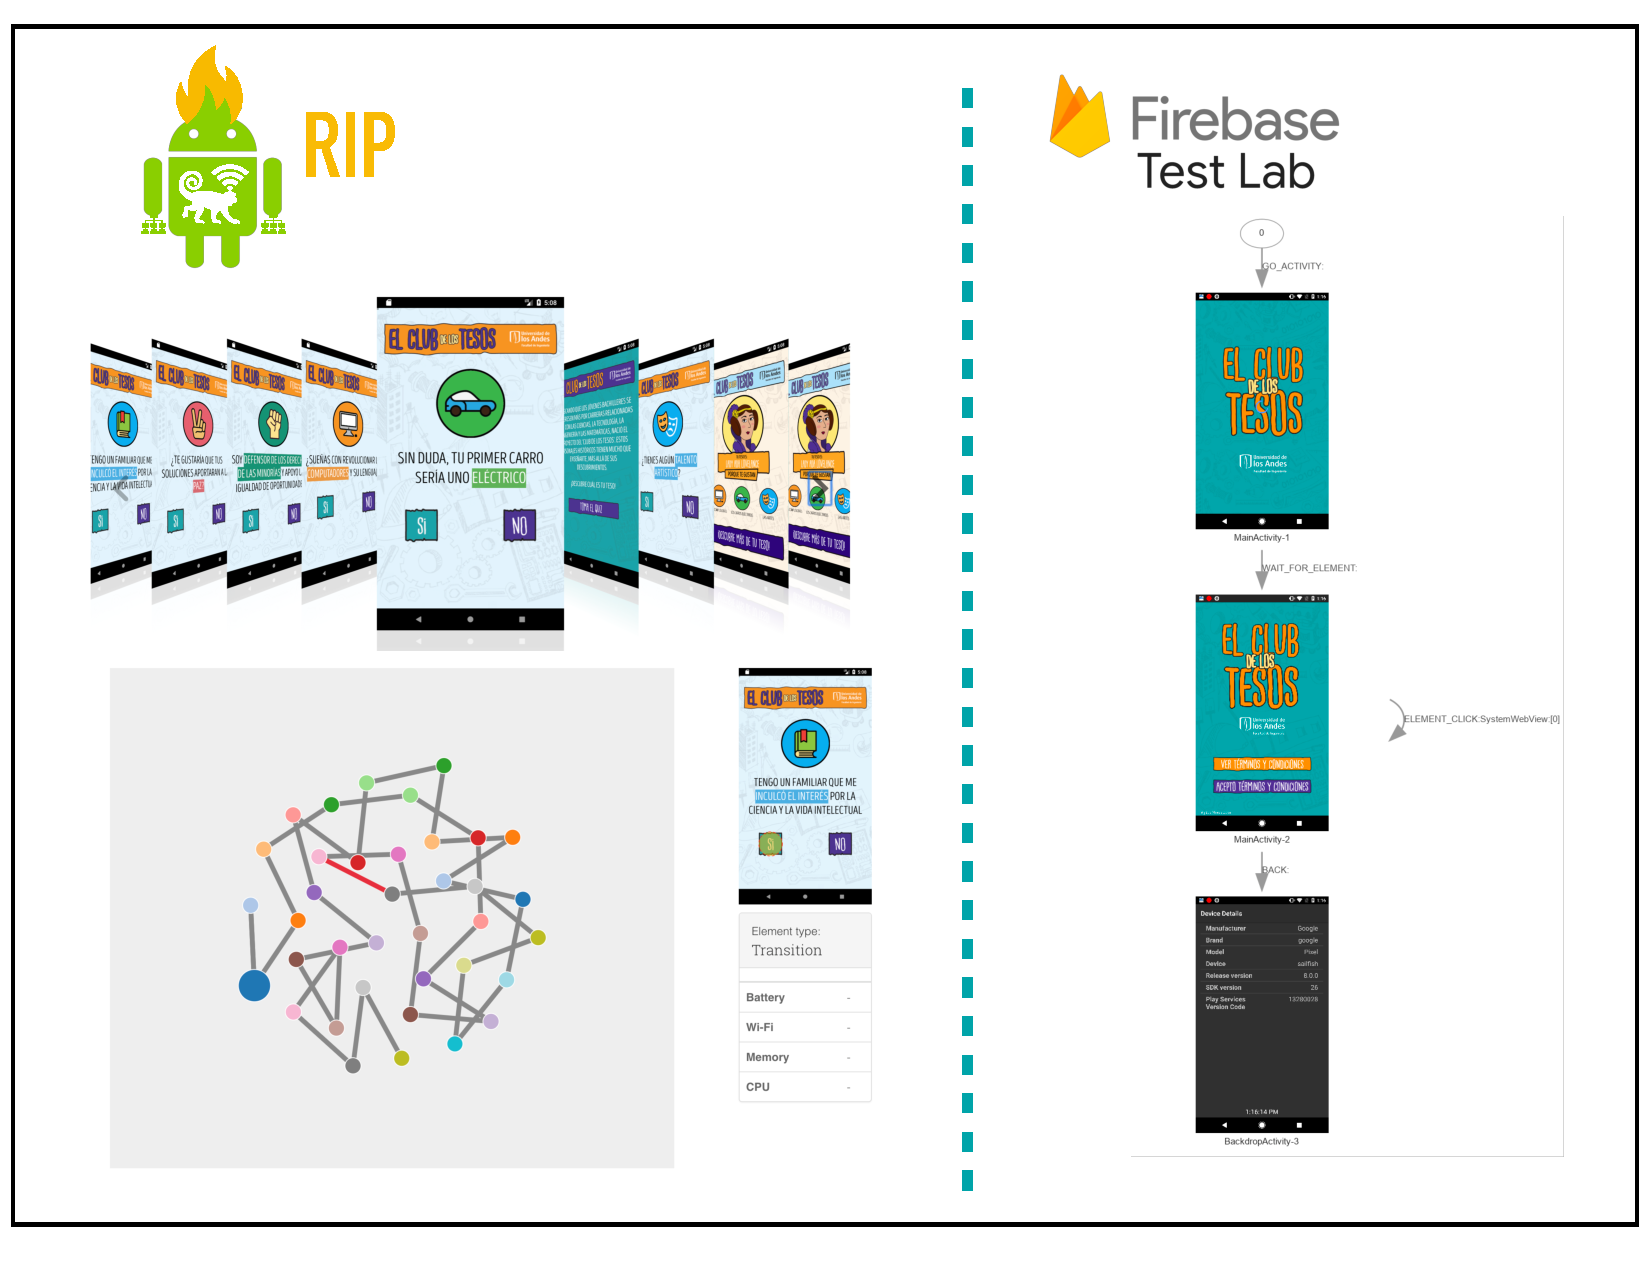
\includegraphics[width=1\textwidth]{img/ripFirebase.pdf}
	\vspace{-0.5cm}
	\caption{Comparison of a hybrid app exploration between RIP and Firebase Test Lab Robo. Firebase only found 2 states of the app: the main screen and the splash image}
	
	\label{ripFirebase}
\end{figure} 

\begin{tcolorbox}[title= \textit{\textbf{RQ$_2$}} How accurate is the \textit{state discovery algorithm} implemented in RIP when compared to state-of-the art tools?]
	Still performance of \textbf{RIP} exploring native applications is lower than existing baseline tools' (based only on GUI ripping), enabling contextual changes in exploration allows \textbf{RIP} to find states that these tools are not able to detect. 
	
	Our tool bridges the gap of ripping hybrid apps, and is the first approach that focuses in exploring dynamically these applications. \textbf{RIP} outperforms industry and academy state of the art tools in the exploration of hybrid apps in terms of detecting new states and not including repeated states in the crawl graph. 
\end{tcolorbox}

\section{\textbf{RQ$_3$} Is RIP suitable to detect crashes and bugs in Android apps?}

To answer \textit{\textbf{RQ$_3$}}, a third case study was carried out in parallel to the experiments of \textit{\textbf{RQ$_2$}}. While exploring each one of the applications, the number of crashes was obtained from \textbf{RIP}, Firebase and Monkey. Crashes from Monkey were extracted manually from the Monkey's log because it does not report aggregated results. In addition, DroidBot was not included in this case study because it neither report crashes nor bugs.

In the complete set of applications, Monkey found one crash in a native application. During the execution of Monkey in hybrid applications, it was able to triggered events that caused ANRs and HTTP errors, however, it was not able to register them because Monkey only detect native crashes.

In native apps, RIP found 2 crashes related to contextual changes (turning on airplane mode) These crashes occurred when the device was connected to Internet and lost connection while executing a background download task. In hybrid applications, RIP found a series of crashes which are presented in the Figure \ref{crashes}. It found crashes in 40 \% of the hybrid applications presented in the list. These crashes include HTTP 500 errors (Internal server errors without description), HTTP 503 errors (Service unavailable) and HTTP 404 errors (not found errors). Some of these crashes are depicted in Figure \ref{ripFindsCrashes}.

\begin{figure}[t]
	\centering
	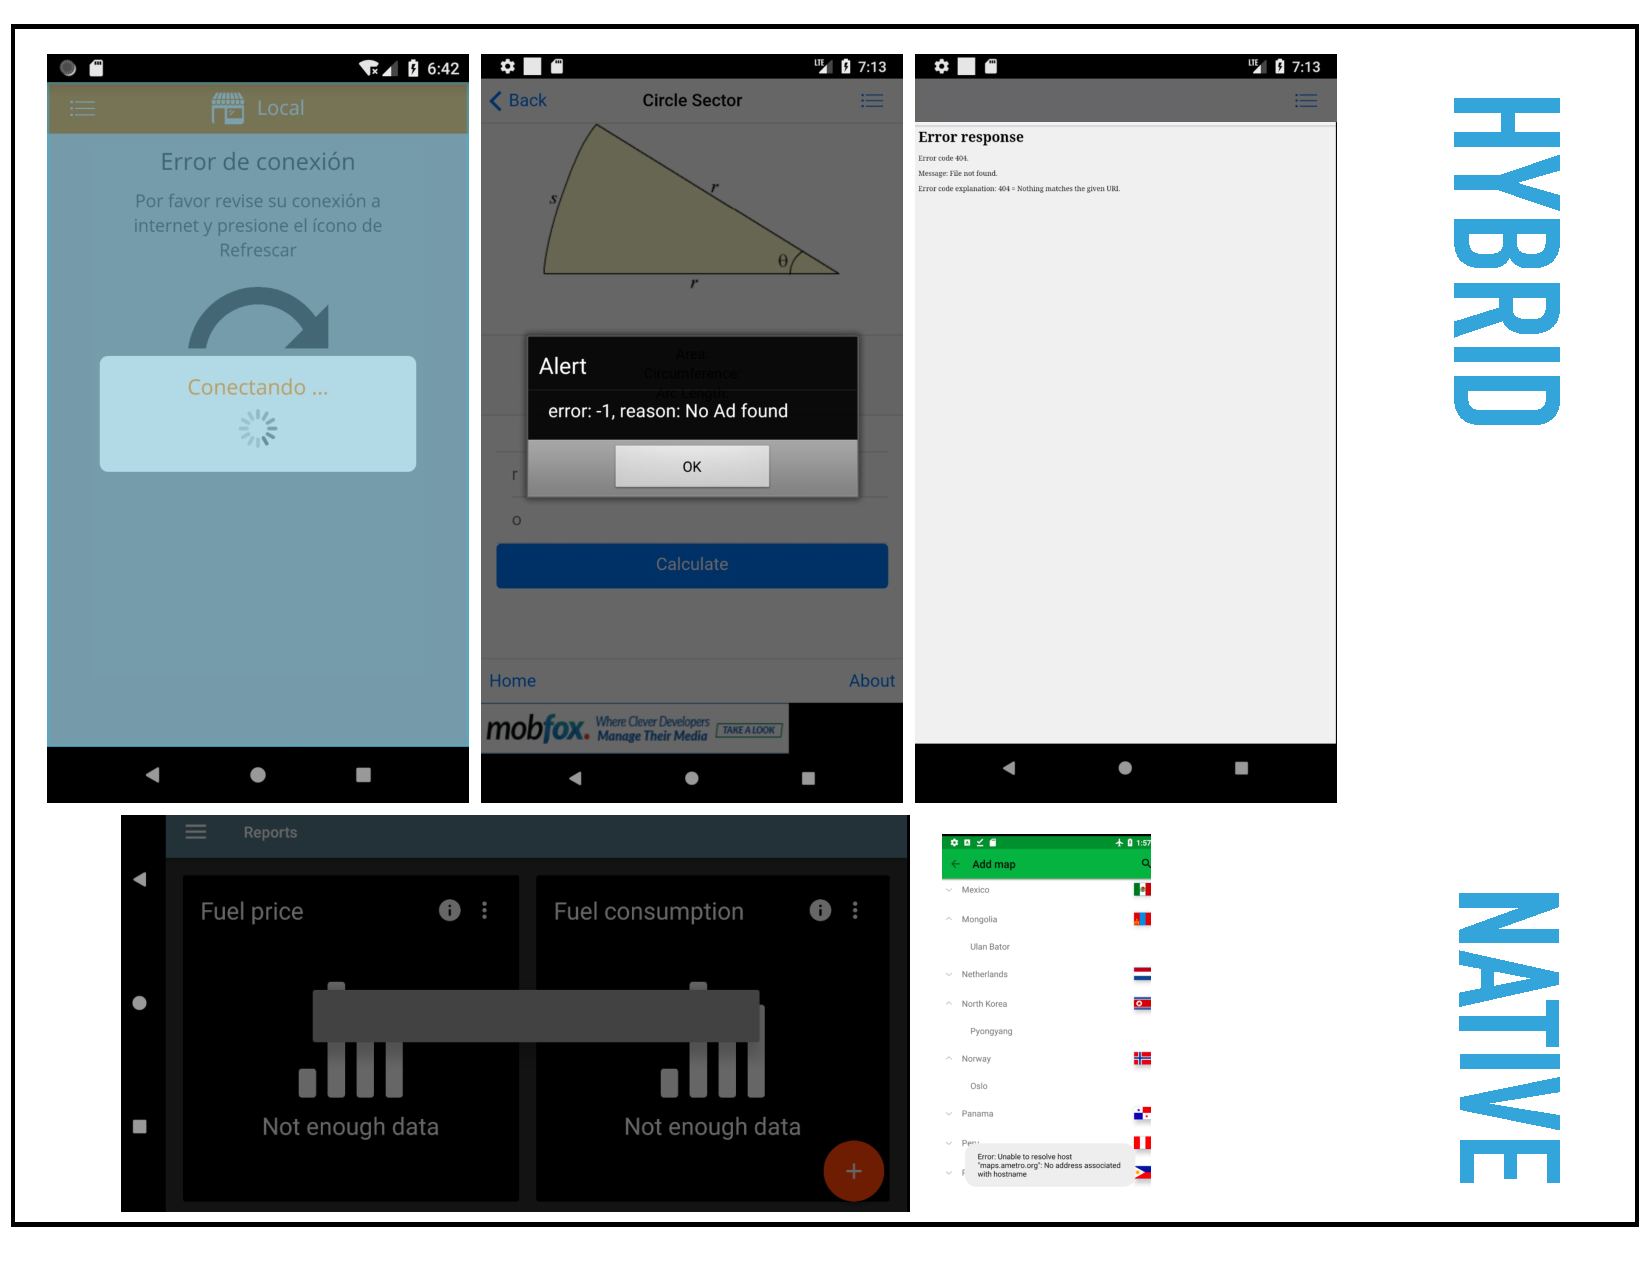
\includegraphics[width=1\textwidth]{img/errorHybrid.pdf}
	\vspace{-0.5cm}
	\caption{Crashes found by \textbf{RIP}}
	\label{ripFindsCrashes}
\end{figure} 


Firebase Test Lab was not able to find crashes in none of the hybrid applications, and did not discover the crashes in the native applications because they were triggered by contextual changes.

We realized that mobile hybrid applications require extensively external web information, and in most cases, the lack of connectivity in the device is not well managed. These scenarios were common, and caused the aforementioned errors.

\begin{figure}[t]
	\centering
	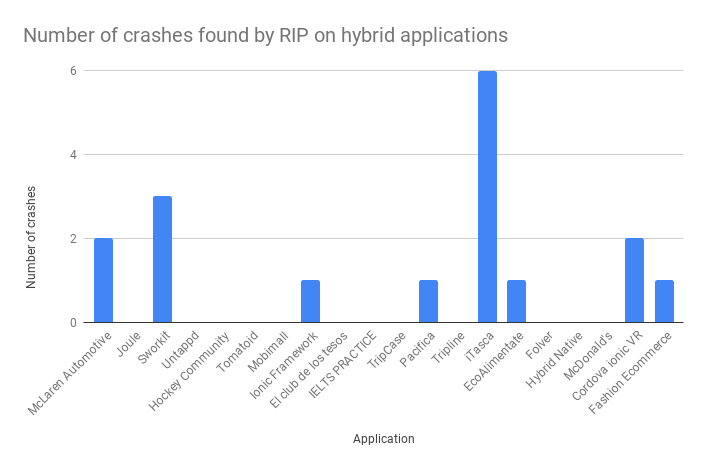
\includegraphics[width=1\textwidth]{img/crashes.png}
	\vspace{-0.5cm}
	\caption{Number of crashes identified by RIP for each hybrid application}.
	
	\label{crashes}
\end{figure} 

\begin{tcolorbox}[title= \textit{\textbf{RQ$_3$}} Is RIP suitable to detect crashes and bugs in Android apps?]
	\textbf{RIP} is able to detect WEB and HTTP crashes from hybrid applications based on the WebView Javascript console whereas native based tools only detect crashes such as \texttt{IOException} or \texttt{OutOfMemoryError}. RIP also detects native crashes reported by the system in the \texttt{logcat}. This combination of web information and native informations gives \textbf{RIP} and advantage over existing tools.
	
\end{tcolorbox}
